\chapter{Flow diagram of the code}

\begin{figure}[H]
    \centering
    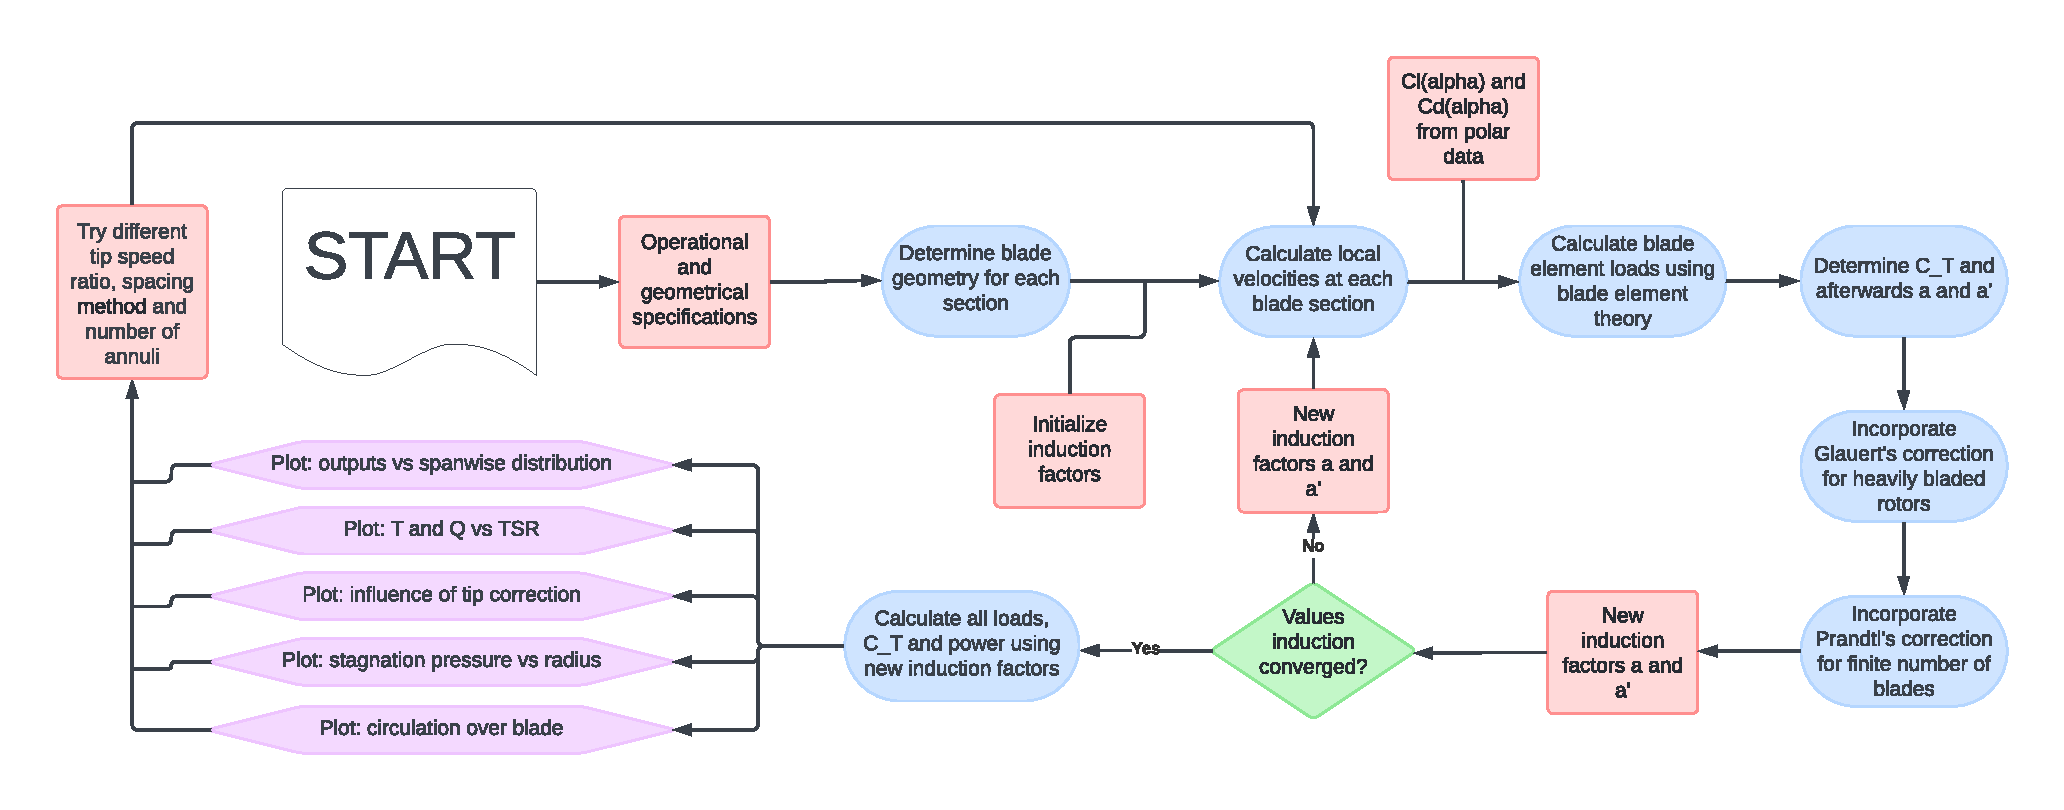
\includegraphics[width=\textwidth]{Figures/Blank diagram.pdf}
    \caption{Flow diagram of the code}
    \label{fig:enter-label}
\end{figure}

\section{Assumptions}
\begin{itemize}
    \item \textbf{Steady Flow:} the flow characteristics are assumed to be independent of time.
    \item \textbf{Inviscid Flow:} the flow is assumed to be inviscid. This means no viscous effects are taken into account.
    \item \textbf{Incompressible Flow:} the flow is assumed to be incompressible. This means the density throughout the streamtube is constant. This enables the use of Bernoulli's equation in locations of a continuous pressure distribution. This also results in the product of area and flow velocity being constant over the flow.
    \item \textbf{2D Flow:} it is assumed that the flow characteristics can accurately be modeled using 2 dimensional flow characteristics.
    \item \textbf{Constant Internal Energy:}  it is assumed that the internal energy within the streamtube is constant so there no radiation, convection or conduction occurring.
    \item \textbf{Independent annulus:} the annuli are considered independently of one another. In reality, flow characteristics on one annulus will influence the characteristics on another (cross flow), this effect is ignored.
    \item \textbf{Circular Discs:} the actuator disc in the model is assumed to be of circular shape. In reality slight changes in the shape could occur, these are neglected.
    \item \textbf{Root-section:} it is assumed that the root section till $r/R = 0.2$ has no influence on the performance of the turbine and can be neglected.
\end{itemize}